% REPLACE: "recall" instead of "factual" knowledge questions
% INTRO: motivate process/structure NOT content

One of the most important tasks for citizens in modern democracies is to vote for candidates who represent their interests and hold their elected officials accountable. While there have been longstanding debates about whether citizens are sufficiently informed to fulfill this task, fundamental issues regarding the measurement of knowledge continue to plague the discipline \citep{mondak2001developing,sturgis2008experiment,pietryka2013analysis}. Most analyses rely on batteries that assess individuals' factual knowledge about political institutions and officeholders \citep[e.g.,][]{carpini1996americans}. Ultimately, these survey questions should cover information that is necessary and/or sufficient for citizens to make competent decisions in a given context \citep[c.f.,][]{lupia2006elitism,lupia2015uninformed}. Yet, determining such a set of items proves to be extremely difficult, especially since there are systematic differences in types of knowledge \citep{barabas2014question}. Even within a given policy area, people may disagree about which facts are crucial for political competence due to inherent value differences \citep{lupia2015uninformed}. Despite these difficulties, most empirical studies rely on a set of off-the-shelf knowledge questions rather than justifying their choices theoretically. As \citet[219]{lupia2006elitism} points out, ``[m]ost political knowledge questions are not derived from a replicable or transparent logic about how their answers bear on a voter's ability to make decisions of a particular quality.'' Furthermore, recall-based measures cannot capture directly how people structure their attitudes and beliefs \citep[e.g.,][]{luskin1987measuring} and thus may not be appropriate indicators of informed preferences \citep{gilens2001political}.

While some scholars contend that simple tests of factual information are nevertheless the best available proxy for political awareness \citep[e.g.,][]{zaller1990political}, others rely on broader conceptualizations of sophistication that incorporate additional dimensions such as education and income \citep[e.g.,][]{jacoby2006value}. Notwithstanding, the fundamental issue remains that knowledge quizzes rarely cover information that is relevant for citizen competence \citep{lupia2006elitism}. In a similar vein, \citet{druckman2014pathologies} describes individual levels of political information as inadequate to measure ``quality opinion'' since there is no consensus about what information is necessary in the first place. Instead, Druckman advocates ``\textit{less} focus on the \textit{content/substance} of opinions [...] and \textit{more} on the \textit{process} and specifically the \textit{motivation} that underlies the formation of those opinions'' \citeyearpar[478, emphasis in the original]{druckman2014pathologies}. 

% Normative democratic theory suggests that voters should hold informed opinions about available candidates and relevant issues before casting a vote.
% The framework proposed herein follows this call by using a person's expressed considerations as an indicator for political sophistication. 
The framework proposed herein follows this call by using a person's open-ended responses to develop an indicator of \textit{discursive sophistication}. The measure examines how respondents discuss their political beliefs in their own words and incorporates information about the number of considerations raised, the relative descriptiveness in word choice, as well as the level of opinionation. The approach is therefore \textit{naive} in that it does not presuppose pieces of information as necessary for political competence but rather examines the respondents' justification of their preferences at face value. Measuring sophistication based on people's verbatim attitude expression provides two major advantages compared to off-the-shelf factual knowledge items: (1) It can easily pinpoint specific areas in politics by incorporating targeted open-ended items in a survey, and (2) it directly captures the extent to which a respondent's beliefs in that area are based on elaborate reasoning.
% Specifically, it assesses whether politically relevant beliefs and opinions are expressed in a more elaborate manner---a question that is not directly discernible when employing off-the-shelf factual knowledge items. 

I validate the measure across multiple data sets by comparing it to conventional factual knowledge scores as predictors of various indicators of competence. While the measures share a considerable amount of variance, they are far from equivalent. Indeed, discursive sophistication is a stronger predictor of turnout and other forms of political participation than traditional metrics. After validating the measurement approach, the paper illustrates how discursive sophistication can help refine previous insights in the literature by re-examining an oft-cited finding in empirical research---the gender gap in political knowledge. Contrary to previous research, I find no evidence for such a gap based on open-ended responses. While women might score lower than men on factual knowledge about political institutions and elites, there are no differences in the complexity of expressed political attitudes.



\section{Opinion Formation and Attitude Expression}

In modern democracies, citizens can engage in politics through various means such as voting in local, state, or federal elections. Depending on the institutional setup, they may also directly decide on specific policies through referenda. In these contexts, we are concerned with the ability of citizens to make high quality decisions in accordance with their underlying interests. Given that it is virtually impossible to determine what information is indeed necessary and/or sufficient to make competent decisions in a given context, scholars should concentrate on whether people are motivated to engage in elaborate reasoning when forming their preferences \citep{druckman2014pathologies}. In previous research, scholars have induced people to engage in in-depth processing by asking them to \textit{justify} their opinions \citep[e.g., by providing specific reasons;][]{kunda1999motivated,redlawsk2002hot,bolsen2014influence,druckman2014pathologies}. In an analogous way, we can examine \textit{how} citizens justify their preferences in order to evaluate whether they engaged in elaborate and sophisticated reasoning \citep[see also][]{rosenberg1988structure,rosenberg1988political}. If respondents are motivated and able to engage in in-depth processing to form quality opinions, they should discuss multiple considerations related to a political issue and show awareness of arguments for and against certain positions \citep{cappella2002argument}. Rather than trying to develop recall items that presupposes a set of facts as necessary for political competence, I therefore analyze \textit{how} individuals discuss their preferences related to a given political task. A similar argument is made in a recent study by \citet{colombo2016justifications}, which investigates the competence of Swiss citizens voting in policy referenda. Analyzing data from thirty-four ballot decisions, the author examines the voters' ``capacity to justify political decisions with policy-related arguments as a possible conceptualization of citizen competence in direct democracy'' \citep[3]{colombo2016justifications}.

This approach is consistent with influential theoretical accounts of political sophistication which focus on the \textit{structure} of belief systems. For example, \citet{converse1964nature} emphasizes the importance of the level of conceptualization as the main characteristic of sophistication rather than isolated pieces of factual information. Similarly, \citet{tetlock1983cognitive,tetlock1993cognitive} uses the term \textsl{integrative complexity} to describe the degree to which considerations related to an issue are interconnected. \citet{luskin1987measuring} also defines political sophistication based on the structure of individual belief systems, arguing that they can vary on three separate dimensions: (1) their \textsl{size} -- i.e. the number of cognitions, (2) their \textsl{range} -- i.e. the dispersion of cognition over categories, and (3) their \textsl{constraint} -- i.e. the extent to which cognitions are interconnected in a meaningful way. Political sophistication, in turn, is seen as the conjunction of these dimensions: ``A person is politically sophisticated to the extent to which his or her [political belief system] is large, wide-ranging, and highly constrained.'' \citep[860]{luskin1987measuring}.

Overall, this body of work suggests that differences in sophistication should be reflected in the way individuals describe and justify their political beliefs. Crucially, a measure of sophistication that is based on how individuals discuss their preferences in their own words can be directly applied in various settings to target specific political tasks such as choosing between candidates, parties, or policy propositions. Rather than having to devise a new set of questions that attempt to capture information necessary to make competent decisions, we can simply analyze how respondents elaborate on their related preferences in verbatim.


\section{Measuring Discursive Sophistication}

How would a politically sophisticated person who engages in in-depth processing discuss his or her views compared to a less informed individual? Consider a survey where respondents are asked to describe their attitudes toward specific policies or candidates running for office in a set of open-ended items. In such a scenario, the structure of individual political belief systems (i.e., size, range, and constraint) as well as the level of motivation to engage in more elaborate reasoning should be reflected in their verbatim responses. In the following, I discuss three different attributes of open-ended survey responses that should be indicative of sophistication in attitude expression.

First of all, sophisticated individuals should be able to elaborate more on their political attitudes. If people possess a large, wide-ranging, and constrained belief system, they should be able to recall a large number of \textit{considerations} related to political actors or issues. I rely on the structural topic model framework \citep{roberts2014structural} to extract the number of topics mentioned by each respondent in a survey.\footnote{See below for more information on the set of open-ended responses, pre-processing choices, as well as on the topic model specification.} First, denote $\mathcal{W}_i$ as the set of words contained in a response of individual $i$. Each word $w\in\mathcal{W}_i$ is assigned to a topic $t^* \in \{1,...,T\} $, such that $P(t^*|w,X_i) > P(t|w,X_i) \forall t\neq t^*$.\footnote{Note that $P(t|w,X_i)=\dfrac{P(w|t)P(t|X_i)}{P(w|X_i)}$. In the context of structural topic models, $X_i$ denotes the covariates used to predict individual topic prevalence \citep[see][for details]{roberts2014structural}.} In other words, each unique term in a response is assigned to the topic that has the highest likelihood of having generated that term, given the model. The set of topics that are mentioned by respondent $i$ across all words in $\mathcal{W}_i$ can then be denoted as $\mathcal{T}^*_i$ and the number of considerations can be written as:
\begin{equation}
\text{considerations}_i = \dfrac{|\mathcal{T}^*_i|}{\max_i|\mathcal{T}^*_i|}.
\end{equation}
The measure is re-scaled to range from zero to one by dividing raw count of topics by the maximum number of topics observed across individuals.

However, sophisticated respondents should not only be able to mention a larger number of raw considerations when discussing politics. The level of sophistication should also be reflected in the \textit{word choice} describing the underlying issues. Individuals who possess a constrained system of beliefs should be more inclined to use terms that are highly descriptive of a given topic (e.g., the \textit{economy} or \textit{taxes}) rather than broad terms that could be attributed to any topic. Highly descriptive word choice is conceptualized as the sum of term likelihoods $P(w|t^*)$ given topic assignments over the entire set of words in $\mathcal{W}_i$:
\begin{equation}
\text{word choice}_i = \dfrac{\sum_{\mathcal{W}_i} P(w|t^*)}{\max_i\left[\sum_{\mathcal{W}_i} P(w|t^*)\right]}
\end{equation}
Again, the measure is re-scaled to range from zero to one by dividing all values by the empirical maximum observed across all individuals in the data.

Lastly, sophisticated individuals should hold opinions about each political actor or policy that they are asked to discuss. As such, sophisticates should be able to express their attitudes towards each open-ended probe in terms of both approval or disapproval. Responses that reflect high levels of sophistication should therefore display a greater level of \textit{opinionation}, which is conceptualized as the diversity of relative lengths for each open-ended response (specified as the Shannon entropy):
\begin{equation}
\text{opinionation}_i = \dfrac{-\sum_{j=1}^J p_{ij} \ln p_{ij}}{\ln J}
\end{equation}
where $p_{ij}$ is the proportion of words in the response of individual $i$ to question $j\in \{1,...,J\}$ relative to the overall size of the individuals' response. The variable ranges from 0 (only one question was answered) to 1 (all questions were answered with the same word length per answer).

Together, the three measures form a composite metric of sophistication in political attitude expression by calculating their respective average for each respondent. Like each individual component, the resulting \textit{discursive sophistication} score ranges from 0 to 1:
\begin{equation}
\text{discursive sophistication}_i = \tfrac{1}{3}(\text{considerations}_i + \text{word choice}_i + \text{opinionation}_i).
\end{equation}
Overall, a highly sophisticated individual can be expected to respond to a set of open-ended items by giving a more elaborate response that focuses on multiple considerations using terms that are highly descriptive of each topic and addresses his or her attitudes towards all relevant political actors or policies more or less equally.\footnote{Note that this approach differs from recent work on sophistication in speeches and other sources of political texts \citep[e.g.,][]{spirling2016democratization,benoit2017measuring} as it explicitly tries to capture complexity independent of pure linguistic style.}


\section{An Overview of Data Sources and Open Ended Items}
% CUTS: This section should start on page 6

The measure of discursive sophistication is validated using multiple surveys employing different sets of open-ended questions. Each survey focuses on sophistication in the context of distinct political tasks, namely the evaluation of (1) candidates running for public office, (2) broad issue areas such as health care and gun legislation, and (3) policy referenda. The data sets and items used to compute discursive sophistication are briefly described below.\footnote{See Appendix A for descriptive information on open-ended responses in each dataset, structural topic model results, and individual components of discursive sophistication. Appendix B contains further details on pre-processing steps and modeling choices for the structural topic models as well as robustness checks, which include preText analyses proposed by \citet{denny2018text}.}


\subsection{2012 \& 2016 American National Election Study}
The main analyses are based on the 2012 and 2016 wave of the American National Election Study (ANES), which consist of a representative survey of about 5000 adults in the months before the US Presidential election in each year. About 2000 respondents in both waves participated in face-to-face interviews while the remaining respondents filled out the survey online. For the purpose of the present analyses, I rely on the pooled datasets while controlling for differences in survey mode. The measure of discursive sophistication is based on open-ended questions in which respondents were asked in the pre-election wave of the survey to list anything in particular that they like/dislike about the Democratic/Republican party as well as anything that might make them vote/not vote for either of the Presidential candidates. They were probed by the interviewer asking ``anything else?'' until the respondent answered ``no.'' Overall, there are a total number of 8 open-ended responses where individuals described their beliefs and attitudes towards political actors. Individuals who did not respond to all of the open-ended items (420 in 2012; 204 in 2016), or who responded in Spanish (228 in 2012; 43 in 2016), were excluded from the analysis.


\subsection{2015 YouGov Survey}
In order to replicate and extend the main analyses, I rely on a separate nationally representative survey employing an alternative set of open-ended responses. The data was collected by YouGov in December 2015 and contains responses of 1000 U.S. citizens.\footnote{See \citet{clifford2016cheating} for details on the study.} As part of this study, respondents were asked to describe their attitudes towards two prominent political issues that were discussed frequently in the media. First, they were asked in a closed format whether they favor or oppose stricter gun laws. Subsequently, they were asked to respond to the following two questions:
\begin{itemize}\setlength\itemsep{0em}
\item Still thinking about the question you just answered, what thoughts came to mind while you were answering that question? Please try to list everything that came to mind.
\item Thinking about the mass shootings that have occurred in the U.S. in the last few years, what factors do you think are responsible for the shootings?
\end{itemize}
Second, the respondents reported on their attitudes towards the Affordable Care Act in a closed format and were then asked to elaborate in their own words by answering the following questions:
\begin{itemize}\setlength\itemsep{0em}
\item Still thinking about the question you just answered, what thoughts came to mind while you were answering that question? Please try to list everything that came to mind.
\item For decades, experts have observed that the United States spends far more per person on health care than any other country. However, the U.S. falls behind on most measures of health care outcomes, such as life expectancy. What factors do you think are responsible for the state of our health care system?
\end{itemize}
Here, discursive sophistication is computed based on the verbatim responses to the four preceding questions using the same procedures described above. Compared to the open-ended likes/dislikes items included in the 2012 and 2016 ANES, the questions directly address considerations related to specific policy issues that were prominent in the political discourse at the time of the survey. Respondents who did not provide an answer to any of the open-ended questions were removed from the analysis (48).


\subsection{Swiss Referendum Survey}
Lastly, I examine survey data on Swiss citizens justifying their vote choices on multiple referenda used in the analyses by \citet{colombo2016justifications}. The author compiled a data set of cross-sectional surveys administered in Switzerland after national popular votes on multiple policy propositions. The original surveys were conducted as representative samples after each of thirty-four national policy votes that were held between 2008 and 2012 resulting in a total of about 27,000 observations. However, respondents were only asked to justify their decision for or against a given proposition in verbatim if they participated in the vote in the first place. As such, 4,917 individuals in the data set did not provide an open-ended response. The remaining respondents were asked to describe the main reason as well as additional justifications for their decision in two separate items. As before, discursive sophistication is computed based on the verbatim responses to both questions.
% QUESTION wording for Swiss study?



\section{A First Look at Discursive Sophistication}

Before turning to the validation, I begin by directly comparing discursive sophistication to alternative metrics of political knowledge in the 2012 and 2016 ANES. The standard approach to measure political knowledge in surveys is to ask a set of factual questions about political institutions. The ANES surveys include such a basic item battery, inquiring for example about the number of times an individual can be elected President of the United States, or how the current U.S. federal budget deficit compares to the deficit in the 1990s. I combine responses on these items to form an additive index of \textit{factual knowledge} about politics. As an additional benchmark, I consider \textit{interviewer assessments} of each respondent's political sophistication  (c.f., \citealt{bartels2005homer} for an example of a study that relies on interviewer assessments; but see also \citealt{ryan2011accuracy}).\footnote{Interviewer assessments were only recorded in the face-to-face sample of the ANES.}

\begin{figure*}[h]
    \centering
    \begin{subfigure}[t]{0.5\textwidth}
        \centering
        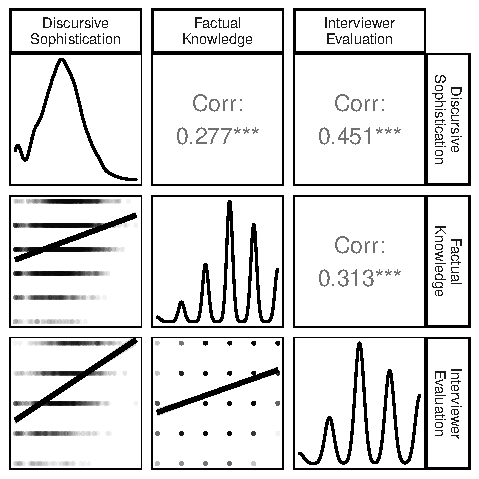
\includegraphics{/data/Dropbox/Uni/Projects/2016/knowledge/fig/anes2012_corplot.pdf}
        \caption{2012 ANES}
    \end{subfigure}%
    ~ 
    \begin{subfigure}[t]{0.5\textwidth}
        \centering
        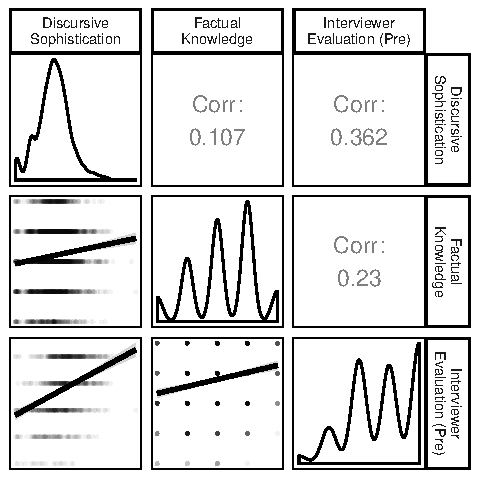
\includegraphics{/data/Dropbox/Uni/Projects/2016/knowledge/fig/anes2016_corplot.pdf}
        \caption{2016 ANES}
    \end{subfigure}
    \caption[Correlation matrix of conventional political knowledge metrics and discursive sophistication]{Correlation matrix of conventional political knowledge metrics and discursive sophistication. The plots on the diagonal display univariate densities for each variable. The panels in the lower triangular display the scatter plot of two measures as well as a linear fit. The upper triangular displays the correlation coefficient. All correlations reported are statistically significant with $p<.05$.}\label{fig:corplot}
\end{figure*}

Figure~\ref{fig:corplot} compares discursive sophistication to the conventional knowledge metrics for both surveys. Each figure presents scatterplots between individual measures (lower triangular), univariate densities (diagonal), and correlation coefficients (upper triangular). The measure of discursive sophistication is positively correlated with both conventional metrics while capturing some additional variation. Interestingly, there is a stronger correlation between discursive sophistication and interviewer evaluations than between factual knowledge and interviewer evaluations ($r=.447$ vs. $r=.313$ in 2012, and $r=.351$ vs. $r=.23$ in 2016). The open-ended measure therefore captures characteristics that influence subjective assessments of sophistication. Interviewers certainly form their impressions throughout the entire survey, but a respondent's verbatim answers seems to be more influential for subsequent knowledge assessments than a respondent's performance on the factual knowledge questions.

Overall, while discursive sophistication and the alternative measures are clearly correlated, the relationship between each metric is far from perfect. To provide some intuition whether the variation in discursive sophistication is theoretically meaningful, I present an example of open-ended responses of two individuals in the 2016 ANES who identified as Republicans and scored equally on the factual knowledge score (3 out of 4 correct responses), but varied highly in discursive sophistication. The results are presented in Table~\ref{tab:ex1}.

\begin{table}[ht]\footnotesize\centering
\begin{tabular}{l|p{6.3cm}|p{6.3cm}}
\toprule
	& A: Low Sophistication Response & B: High Sophistication Response \\ \midrule
Clinton (+)		& 																& Politician. \\\hdashline
Clinton (-)		& The fact that she has links to Al-Qaeda. 						& Caught in lies. \\\hdashline
Trump (+)		& 																& Says what he thinks. \\\hdashline
Trump (-)		& He is going to start a civil war. I feel like he is racist. 	& Reality TV star, poor businessman \\\hdashline
Democrats (+)	& 																& Middle class minded. \\\hdashline
Democrats (-)	& 																& Too many handouts. \\\hdashline
Republicans (+)	& 																& Economic growth conscious. \\\hdashline
Republicans (-)	& 																& For the big business. \\\midrule
Disc. Soph. 	& 0.159 														& 0.465 \\\bottomrule

 \end{tabular}
\caption{Example of open-ended responses for low and high scores on discursive sophistication with equal factual knowledge scores (3 out of 4 correct responses). Column A displays the verbatim responses of an individual who scored low on discursive sophistication and column B displays the verbatim responses of an individual who scored high on the open-ended measure. Each row represents one of the likes/dislikes items included in the analysis. Note that the responses in this table were slightly redacted for readability (spelling errors removed, etc.).}\label{tab:ex1}
\end{table}

Each row in the table represents one of the open-ended responses (like/dislike for each candidate/party). Column A displays the responses of an individual who scored low on discursive sophistication and column B displays the responses of a high scoring individual. Cells are empty if a respondent refused to provide a response. Even though both individuals are measured to have equal factual political knowledge, there are systematic differences in their response behavior that can be attributed to their political sophistication. Overall, respondent A provided a less elaborate response, only focused on a narrow range of issues, and only reported attitudes on two items. Irrespective of whether one agrees with the specific statements or whether they are factually accurate (e.g., Clinton's connection to Al-Qaeda), A's response pattern is suggestive of a less sophisticated political belief system and a lower level of motivation to engage in in-depth processing about both parties and candidates. Overall, this initial result suggests that the variation in discursive sophistication captures meaningful differences in response behavior that overlaps with traditional knowledge metrics while displaying some unique variation. The following sections will show that this variation is also politically consequential.



\section{Discursive Sophistication and Political Competence}

I validate the measure of discursive sophistication by directly examining its effects on individual competences to perform political tasks in modern democracies \citep[c.f.,][]{lupia2006elitism,lupia2015uninformed}. More specifically, I consider the potential role of political sophistication in promoting (1) engagement and participation in politics, (2) the ability to incorporate new information, (3) precise positioning of candidates running for election, (4) well-justified policy preferences, and (5) vote choices that are consistent with underlying interests. In the following, each point will be addressed using one of the three data sets described above.


\subsection{Engagement and Participation in Politics}
Political sophistication is often argued to promote individual engagement and participation in politics. In fact, factual knowledge items have been validated in the past based on their strong relationship with outcomes such as turnout and other forms of participation \citep[c.f.,][230--233]{lupia2015uninformed}. Figure~\ref{fig:knoweff} compares the effects of discursive sophistication and factual knowledge in the 2012 and 2016 ANES on four dependent variables related to political engagement: turnout, non-conventional participation, internal efficacy, and external efficacy. The model predicting turnout is estimated via logistic regression while the estimates for the three remaining dependent variables are based on OLS. Each model equation includes both sophistication measures while controlling for gender, education, income, age, race, religiosity, survey mode (face-to-face vs. online), as well as the Wordsum vocabulary score measuring verbal intelligence.

\begin{figure}[h]\centering
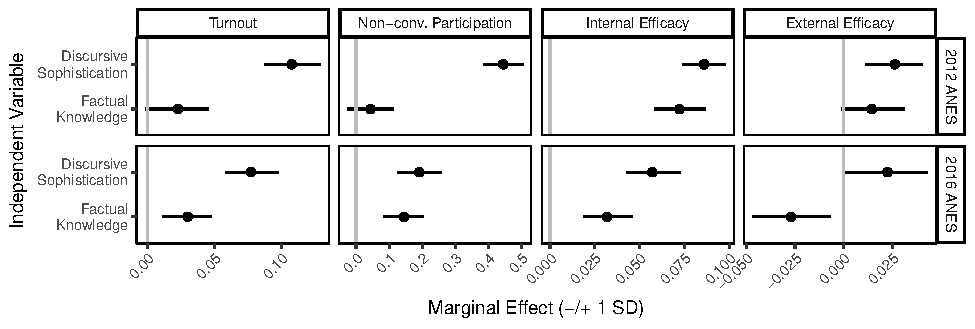
\includegraphics{/data/Dropbox/Uni/Projects/2016/knowledge/fig/knoweff_pres.pdf}
\caption[Effects of sophistication on internal efficacy, external efficacy, non-conventional participation, and turnout in the 2012 and 2016 ANES]{Effects of sophistication on internal efficacy, external efficacy, non-conventional participation, and turnout in the 2012 and 2016 ANES. For each dependent variable, the figure displays the change in expected values after increasing each sophistication measure from -1 to +1 standard deviation from its mean (including 95\% confidence intervals). Model estimates are based on logistic regression (turnout) or OLS (internal efficacy, external efficacy, non-conventional participation). Both sophistication measure are included simultaneously while controlling for gender, education, income, age, race, church attendance, survey mode, and Wordsum vocabulary scores.
%Full model results ar presented in the appendix, Tables \ref{tab:inteff} through \ref{tab:turnout}
}\label{fig:knoweff}
\end{figure}

Each panel displays the expected difference in the respective dependent variable for a two standard deviation increase in each sophistication measure, while holding all other variables constant at their means. Overall, discursive sophistication is a stronger predictor of turnout, non-conventional participation, as well as (to a lesser extent) internal and external efficacy. In the 2012 ANES, the positive effect of factual knowledge on participation is statistically indistinguishable from zero when controlling for discursive sophistication. Furthermore, there is a negative effect of factual knowledge on external efficacy in the 2016 ANES. In contrast, the positive effect of discursive sophistication on external efficacy appears to be more consistent with previous research.


\subsection{Incorporation of New Information}
Competent citizens should not only engage in politics but are also expected to be sufficiently informed about the issues of the day. As such, they have to be attentive to their media environments and incorporate potentially relevant new information about parties, office-holders, and policies. \citet{zaller1990political,zaller1992nature} and others argue that tests of factual information about politics are the best available proxy for awareness. In this analysis I draw on the 2015 YouGov study to explore whether discursive sophistication or factual knowledge serves as a better predictor of people's ability to incorporate new information from media sources. As part of the survey, respondents were asked to read a newspaper article about a fictional infectious disease and were subsequently asked to answer questions about information provided in the article (e.g. regarding symptoms, modes of contraction etc.). I compute an additive index counting the pieces of information that were correctly recalled (\textit{information retrieval}) as a measure of the ability to retrieve information from a news article on a non-partisan issue that is related to public health policies. 

\begin{figure}[h]\centering
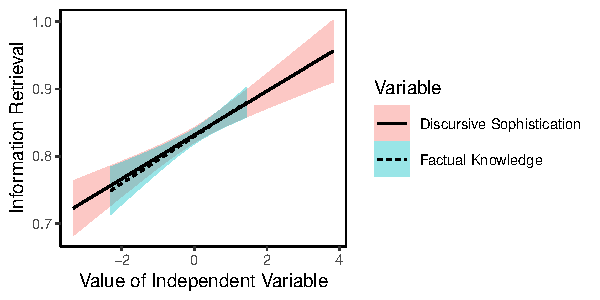
\includegraphics{/data/Dropbox/Uni/Projects/2016/knowledge/fig/yg_disease.pdf}
\caption{Expected disease information retrieval in the 2015 YouGov Study as a function of political sophistication (including 95\% confidence intervals). Estimates are based on a linear regression model controlling for education, income, age, religiosity, gender, and race.}\label{fig:yg_disease}
\end{figure}

Figure~\ref{fig:yg_disease} displays the relationship between political sophistication and disease information retrieval in the 2015 YouGov study. Estimates are based on a linear regression model controlling for education, income, age, religiosity, gender, and race. As a benchmark for discursive sophistication, I again consider the effect of factual knowledge based on a battery of eight items similar to the knowledge questions in the ANES. Both discursive sophistication as well as factual knowledge increase the amount of information individuals are able to recall from a news article discussing a fictional disease. Similar to the previous results, the effects are stronger for discursive sophistication than for factual knowledge scores. The degree to which citizens discuss their own political beliefs in a more elaborate manner is not only a stronger predictor of political engagement but also serves as a better proxy for the ability to incorporate new information about a non-partisan issue (in this case related to public health).


\subsection{Precise Positioning of Candidates}
Citizens who are attentive to politics and able to incorporate new information should ultimately be better informed about the policies put forward by parties and political elites. This is a crucial component of citizen competence in representative democracies since precise knowledge about the policy positions held by candidates who are running for office ultimately allows voters to hold them accountable. Figure~\ref{fig:hetreg} presents the results of multiple heteroskedastic regressions where the error variance in candidate placements on multiple issues included in both ANES waves (general ideology, government spending, defense spending, health insurance policy, job guarantee, government assistance to Blacks, environment vs. jobs trade-off) is a modeled as a function of discursive sophistication as well as factual knowledge \citep[see][for a similar procedure]{jacoby2006value}. More formally, each model for a given candidate placement on a specific policy issue takes the following form:
\begin{align}
y &\sim \text{N}(\mu, \sigma) \\
\mu &= X\beta \\
\log(\sigma) &= Z\gamma,
\end{align}
where $y$ is the vector of policy placements across respondents, $X$ is a matrix of covariates predicting average candidate placements $\mu$ (self-placement, education, income, age, religiosity, gender, race, and survey mode), $Z$ denotes the covariates predicting the error variances $\sigma$ (discursive sophistication, factual knowledge, Wordsum score), and $\beta$ and $\gamma$ are the parameters to be estimated.

\begin{figure}[h]\centering
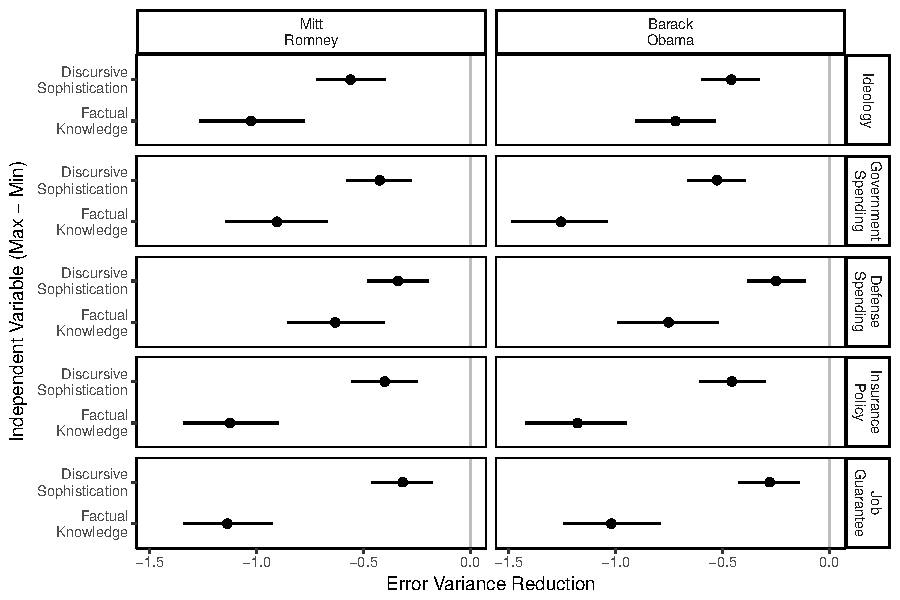
\includegraphics{/data/Dropbox/Uni/Projects/2016/knowledge/fig/hetreg.pdf}
\caption{Error variance reduction in candidate placements on multiple issues in the 2012 and 2016 ANES. The figure displays the difference in estimated error variances after increasing each sophistication measure from -1 to +1 standard deviation from its mean (including 95\% credible intervals). Models are estimated in Stan using non-informative priors.}\label{fig:hetreg}
\end{figure}

The figure displays the estimated reduction in error variances of candidate placements when each sophistication measure is increased by two standard deviations. Larger negative values indicate a stronger reduction in error variances and hence more precise candidate placements. Both factual knowledge and discursive sophistication significantly decrease error variances in policy placements of presidential candidates. Some interesting differences, however, emerge when comparing both waves of the ANES. In the 2012 election, discursive sophistication in open-ended responses was a stronger predictor of precise candidate placements than performance on factual knowledge quizzes across multiple issues. This picture appears to be reversed in the 2016 election, where more elaborate open-ended responses were only weakly predictive of precise candidate placements. This finding may be attributed to idiosyncrasies related to how citizens discuss their preferences for Clinton or Trump as compared to previous candidates, or to higher overall uncertainty about their respective policy positions. Notwithstanding these contextual variations, both factual knowledge and discursive sophistication appear to increase the precision with which individuals place candidates on various policy issues.


\subsection{Well-Justified Policy Preferences}
Beyond keeping track of the candidates' positions, competent citizens should be knowledgeable about the underlying policies themselves and be able to justify their own preferences. Here, I explore the extent to which high levels of discursive sophistication correspond to well-justified policy preferences in open-ended responses. As mentioned above, the Swiss surveys included items that asked respondents to explain why they voted in favor or against a given proposition in multiple policy referenda. To corroborate the face validity of discursive sophistication, I examine whether the measure is related to Colombo's \citeyearpar{colombo2016justifications} manual coding of the respondents' \textit{level of justification}, which directly assessed the content, elaboration, and complexity of open-ended responses.

\begin{figure}[h]\centering
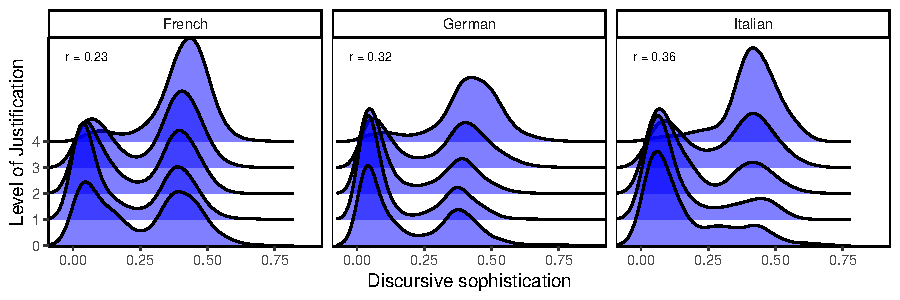
\includegraphics[scale=1]{/data/Dropbox/Uni/Projects/2016/knowledge/fig/swiss_ggridges.pdf}
\caption{Discursive sophistication and manually coded level of justification \citep{colombo2016justifications} in Swiss post-referendum surveys. The plot compares kernel densities of discursive sophistication for each manually coded level of justification.}\label{fig:swiss_ggridges}
\end{figure}

The results are presented in Figure~\ref{fig:swiss_ggridges}. Since the Swiss post-referendum surveys were conducted in three different languages (German, French, and Italian), I computed the measure of discursive sophistication separately for each group of respondents. The figure displays the distribution of discursive sophistication for each level of justification coded by \citet{colombo2016justifications} as well as the correlation coefficients for both respective variables. Across all three language groups, discursive sophistication is systematically higher among respondents with the highest level of justification and both measures are positively correlated ($r=0.29, 0.25$, and $0.35$, respectively). The proposed measure of discursive sophistication therefore shows a high degree of correspondence with individual levels of justification assessed by independent manual coders.


\subsection{Correct Voting}
Ultimately, political sophistication should enable citizens to make high-quality decisions based on informed preferences about relevant issues. The most direct way for citizens in representative democracies to influence policy outcomes in their favor is to cast votes for candidates who best represent their interests. \citet{lau1997voting} proposed a measure of ``correct voting'' that attempts to capture whether citizens are able to choose candidates in accordance with their own values and principles. In other words, correct voting evaluates whether citizens vote for the candidates they would have preferred \textit{had they been fully informed} \citep[see also][]{lau2008exploration,sokhey2012social}. The measure is based on the extent to which a person's vote choice corresponds to a combination of her party identification, issue preferences, and linkages to social groups.\footnote{See Appendix C for more details on the conceptualization of correct voting.} Using both ANES surveys, Figure~\ref{fig:correctvote} examines the effect of political sophistication on the probability to cast such a ``correct'' vote. Estimates are based on logit models where the dependent variable indicates whether the vote choice reported in the post-election wave is considered a correct vote as conceptualized by \citet{lau1997voting} and others.

\begin{figure}[h]\centering
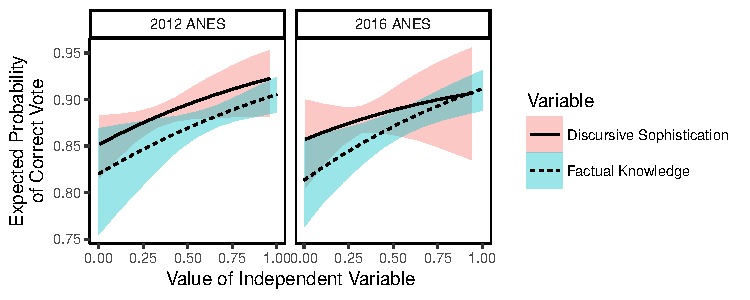
\includegraphics{/data/Dropbox/Uni/Projects/2016/knowledge/fig/correctvote.pdf}
\caption{Predicted probability to cast a correct vote as a function of political sophistication while holding all other variables constant at their respective means (including 95\% confidence intervals). Estimates are based on logit models controlling for education, income, age, religiosity, gender, race, survey mode, and Wordsum vocabulary scores.}\label{fig:correctvote}
\end{figure}

Both, discursive sophistication as well as factual knowledge significantly increase the probability of correct voting. Furthermore, in the 2016 ANES, the effect of discursive sophistication is slightly larger than that of factual knowledge. The degree to which citizens provide more elaborate responses discussing their political preferences proves to be a strong predictor of their ability to cast votes consistent with their underlying values and principles.

Overall, the results presented thus far indicate that discursive sophistication shares common characteristics with factual political knowledge measures. Compared to conventional metrics, the proposed measure performs as least as well as a predictor of essential competences that allow citizens to engage successfully in politics. In fact, discursive sophistication is a stronger predictor of certain outcomes (such as different forms of political participation) than conventional knowledge scores. In the following, I turn to an application to examine how discursive sophistication can help refine important previous insights from the literature on political knowledge.


\section{Application: The Gender Gap in Political Knowledge}

A common finding in public opinion research is the fact that women have lower levels of observed political knowledge than men. For example, \citet{verba1997knowing} report that women score lower on political information, interest, and efficacy, which decreases their respective levels of political participation. Since gender differences in political information and interest can only partly be explained by resource-related factors such as individual levels of education, the authors diagnose a ``genuine difference in the taste for politics'' between men and women, which they suspect to be driven largely by socialization \citep[see also][]{wolak2011roots}. Indeed, \citet[117]{dow2009gender} describes the systematic gender differences in knowledge ``one of the most robust findings in the study of political behavior.''

The discussion revolving around this apparent gender gap is closely intertwined with the methodological debate about measuring political knowledge. For example, \citet{mondak2004knowledge} suggest that women are more likely to report that they do not know the answer to a recall question whereas men are more inclined to guess. Correcting for the systematic differences in the propensity to guess, however, mitigates the gender gap in knowledge but does not eliminate it completely \citep[see also][]{lizotte2009explaining}. Other aspects of the survey context have been shown to affect gender differences in political knowledge. For example, \citet{mcglone2006stereotype} present evidence that the gender gap is exacerbated in an environment that induces stereotype threat, for example if women are aware of the fact that the study focuses on gender differences or if they are interviewed by a male interviewer. However, gender differences are not only induced by \textit{how} researchers ask their questions, but also by the question \textit{content} itself. For example, \citet{dolan2011women} argues that the gap can be closed by focusing on gender-relevant political knowledge items such as information about women's representation in the federal government \citep[see also][]{graber2001processing,fraile2014does,jerit2017revisiting}. Similarly, \citet{stolle2010women} report that the gender gap disappears when people are asked about more practical issues related to the government (e.g., benefits and services).

Overall, the gender gap has been shown to be influenced by how we ask for political information in surveys, as well as the kind of knowledge that is required for a correct response. Indeed, a comprehensive cross-national analysis of election studies in 47 countries between 1996 and 2011 suggests that question format and content account for large portions of the variance of gender disparities in political knowledge \citep{fortin2016cross}.


\subsection{Descriptive Results}
How do men and women compare on the different metrics of political sophistication in the surveys analyzed in the present study? Figure~\ref{fig:meandiff} displays the average levels of discursive sophistication as well as conventional metrics comparing both genders. While we observe a sizable gender gap for factual knowledge in both ANES surveys, this difference disappears for discursive sophistication. These results are replicated in the 2015 YouGov survey. As before, we observe a significant gender gap in factual knowledge which disappears using the discursive measure. Of course, it is important to ask whether this absence of a gender gap in discursive sophistication is theoretically meaningful or rather an artifact of the measurement approach itself. Recall that \citet{colombo2016justifications} manually coded levels of justification in Swiss referendum surveys. The bottom half of Figure~\ref{fig:meandiff} displays her manually coded measure as well as discursive sophistication comparing both genders. Crucially, there are no significant gender differences on \textit{both} metrics across all three languages in the Swiss referendum surveys. The absence of a gender gap is consistent whether open-ended responses are coded manually or using the proposed measure of discursive sophistication.

\begin{figure}[h]\centering
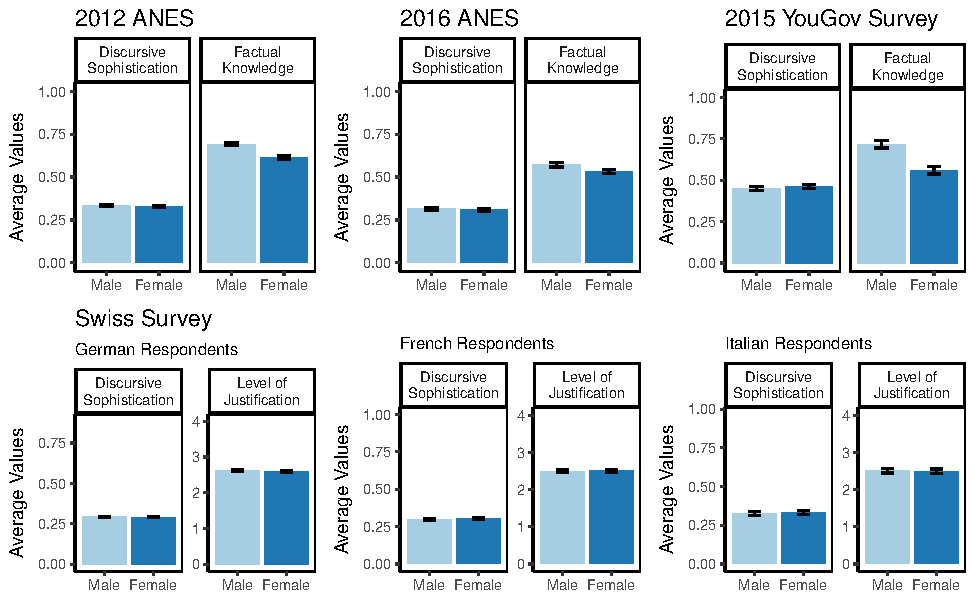
\includegraphics{/data/Dropbox/Uni/Projects/2016/knowledge/fig/meandiff.pdf}
\caption{The gender gap in political sophistication. The figures display mean levels of sophistication for each measure comparing men and women (including 95\% confidence intervals). Gender differences in factual knowledge are statistically significant with $p<.05$.}\label{fig:meandiff}
\end{figure}


\subsection{Controlling for Alternative Explanations}

Prior research suggests that at least part of the gender gap can be attributed to real differences in resources relevant to political information (e.g., education). Accordingly, we need to control for common determinants of political knowledge across all available measures to provide a more comprehensive examination of potential gender differences. Previous studies consistently showed that political knowledge is positively related to high media exposure, frequent political discussions, education, and income. Furthermore, I include age, race, religiosity, and survey mode (face-to-face vs. online) as additional control variables. Figure~\ref{fig:determinants} displays the coefficients of regression models with each knowledge/sophistication measure as the dependent variable.

\begin{figure}[h]\centering
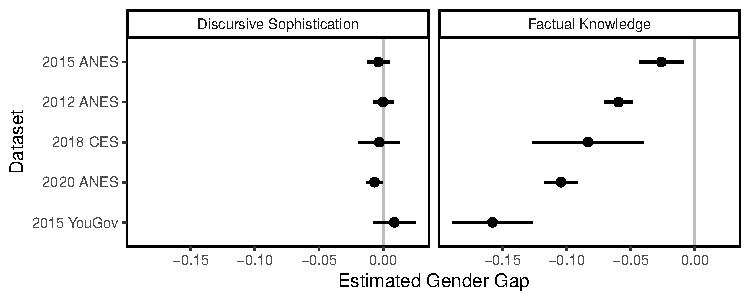
\includegraphics{/data/Dropbox/Uni/Projects/2016/knowledge/fig/determinants.pdf}
\caption{Common determinants of political sophistication. Estimates are OLS regression coefficients with 95\% confidence intervals. Dependent variables are discursive sophistication as well as conventional metrics of political knowledge.
%Full model results are presented in the appendix, Table~\ref{tab:determinants}
}\label{fig:determinants}
\end{figure}

After controlling for common determinants in the 2012 and 2016 ANES, discursive sophistication again reveals no significant differences between men and women. On the other hand, we still observe the gender gap using conventional political knowledge metrics. As such, women might not score as highly on political quizzes, but they do not differ substantially in complexity and sophistication when they describe their political preferences.

The patterns for the remaining determinants are quite similar across different dependent variables. Knowledge and sophistication is significantly higher among respondents who are more exposed to political news media, discuss politics frequently, are more educated, and have higher income.\footnote{An interesting deviation, however, is the effect of survey mode. Respondents in online surveys score significantly higher on factual knowledge than in face-to-face interviews. This difference can be attributed to the fact that individuals are able to look up answers for factual knowledge questions while taking an online survey \citep[c.f.,][]{clifford2016cheating}. For discursive sophistication, on the other hand, individuals perform better in the face-to-face survey. Open-ended answers in online surveys may be less elaborate because respondents have to manually type their responses.} Overall, the finding that determinants of political sophistication are consistent across models lends additional validity to the open-ended measure. As before, this result is replicated when examining data from the 2015 YouGov survey: men do not perform better than women on discursive sophistication in a multivariate setting. The gender gap in factual political knowledge, however, persists and is substantively as well as statistically significant. The remaining determinants of sophistication/knowledge are largely similar across measures.

To summarize, we only observe a significant gender gap when looking at conventional recall-based measures, a result that previous research (at least partly) attributed to the content (i.e., focusing on issues that are less relevant to women) and format (i.e., stereotype-threat and guessing) of the question batteries. For the alternative measure---discursive sophistication---any evidence for systematic differences between men and women disappears.


\subsection{Explaining the (Lack of the) Gender Gap}
If it is the case that women are able to close the gender gap in discursive sophistication because they are able to focus on different considerations that are salient to them when discussing their political preferences, we should observe systematic variation in the issues men and women discuss in open-ended responses. Based on the structural topic model used to compute discursive sophistication, I now examine the subset of topics that showed the largest absolute gender difference in topic prevalence in the 2012 and 2016 ANES. The results are displayed in Figure~\ref{fig:stm_gender}.

\begin{figure}[h]\centering
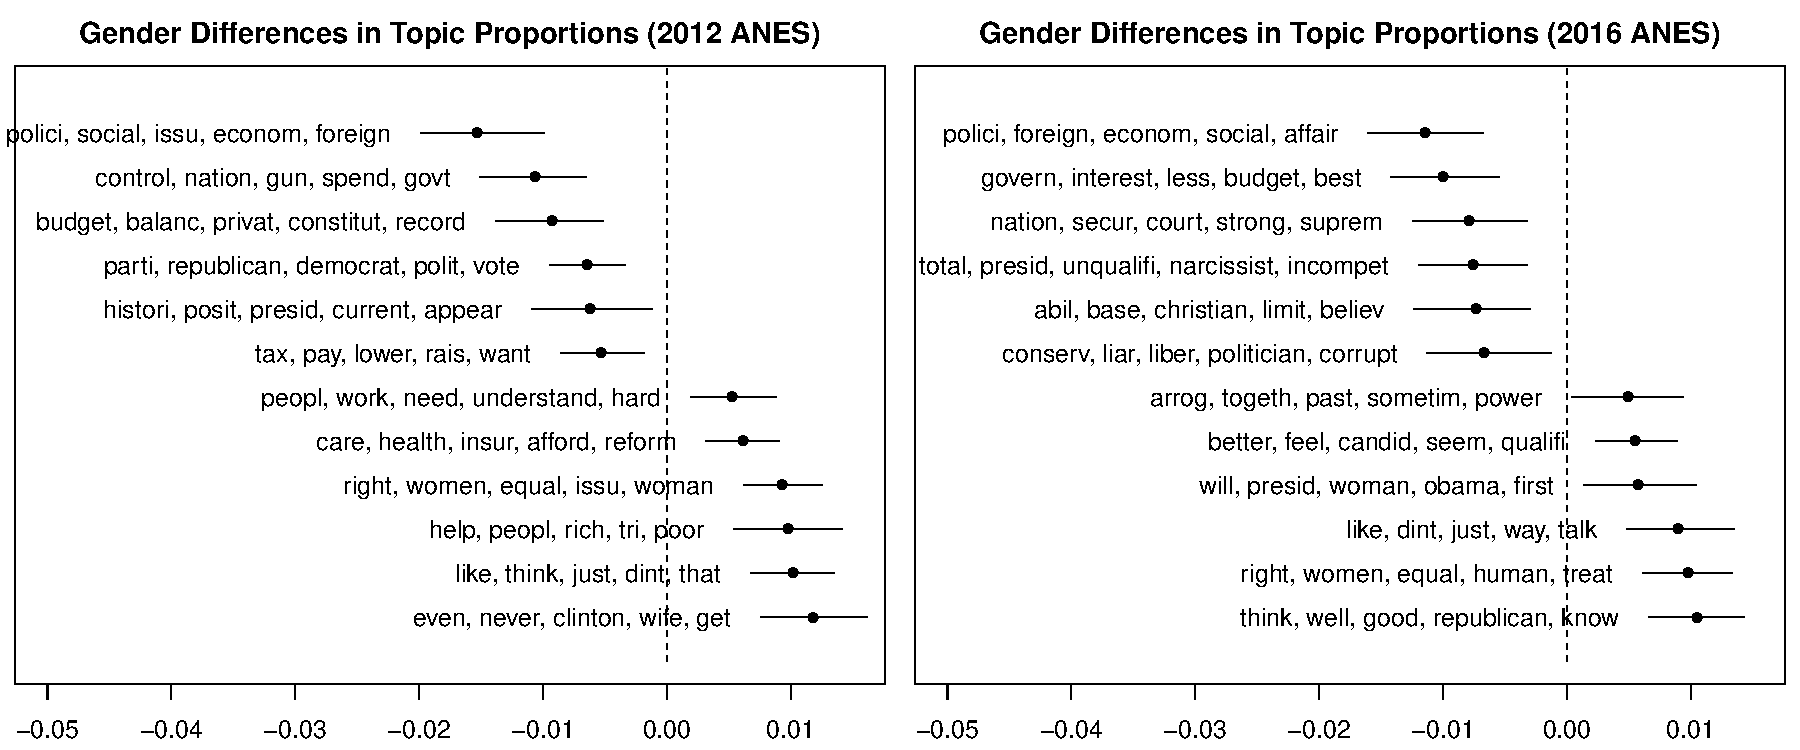
\includegraphics[width=\textwidth]{/data/Dropbox/Uni/Projects/2016/knowledge/fig/stm_gender.pdf}
\caption{Gender differences in topic proportions based on the structural topic model used to compute discursive sophistication (including 95\% confidence intervals). Coefficients indicate the difference in predicted topic prevalence among men and women; positive values indicate higher prevalence among women. Labels are based on the five highest probability terms related to the topic.
%Full model results are presented in the appendix, Table~\ref{tab:determinants}
}\label{fig:stm_gender}
\end{figure}

Positive coefficients indicate that women are more likely than men to mention a given topic, and vice versa. As such, the top five topics are more prevalent among men and the bottom five have a higher probability to be mentioned by women. Each coefficient is labeled with the five highest probability terms related to the topic to illustrate its content. Across both ANES studies, women were less likely than men to discuss foreign affairs, economic issues, or the Supreme Court. Instead, they focused on issues related to women's rights, equality, or health care. The considerations taken into account by women when discussing their political preferences are therefore clearly different from men's and---crucially---the issues raised by men happen to be more aligned with what political scientists often deem as necessary information (i.e., pertaining to the economy, institutions, elites, etc.). Yet, from a normative perspective, there is no reason to assume that one set of issues should be more important for citizens when forming their political preferences and making competent voting decisions.



\section{Conclusion}
% What is a competent citizen? One who has good reasons for his or her attitudes... we can measure that when examining how repondents talk about their political beliefs.

Political scientists should worry less about pure levels of \textit{factual knowledge} and instead focus on the necessary conditions for individuals to make \textit{competent} decisions. Competence in the context of political decision-making and voting requires citizens to hold informed attitudes about their representatives. Factual knowledge about political institutions might be a useful proxy for competence in certain scenarios. However, it cannot address directly whether individuals hold well-considered opinions about political actors they try to hold accountable. In comparison, the measure of discursive sophistication proposed here is agnostic about the specific contents of individual beliefs, but directly captures the complexity of individual attitude expressions.

The findings presented in this paper show that conventional knowledge indices and the discursive measure share a substantial amount of variance. However, they are far from being identical and capture different aspects of sophistication. Most importantly, using the discursive measure, any evidence for the gender gap commonly reported using factual knowledge scales disappears. Women might know fewer facts about political institutions, but they do not differ substantively in the complexity of their expressed political beliefs. The fact that women perform just as well as men on discursive sophistication across various surveys can be attributed to the fact that they focus on different considerations when evaluating political parties and candidates. This issue has long been recognized in the literature \citep[e.g.,][]{graber2001processing,dolan2011women}, but it cannot be properly addressed while relying exclusively on off-the-shelf political knowledge batteries. As mentioned before, \citet{zaller1992nature} and others made the argument that testing for factual information provides the best measure of political awareness as it captures ``what has actually gotten into people's minds, which, in turn, is critical for intellectual engagement with politics'' (21). The results presented in this paper suggest that a direct examination of open-ended responses provides a viable alternative approach.

% DISCUSS: highlight the advantages of the measure, also regarding the ability to find policy areas that are less gender biased.

% DISCUSS manual coding as alternative? However, manual coding of open-ended responses as employed by \citet{colombo2016justifications} is not always feasible in the context of large-scale surveys, since it can be labor-intensive and requires extensive contextual knowledge, such as high levels of language proficiency.\footnote{The Swiss surveys in Colombo's \citeyearpar{colombo2016justifications} study were conducted in three different languages: German, French, and Italian.} Furthermore, knowledge assessments can be biased by the level of political agreement between individuals \citep{ryan2011accuracy}. As such, I present an alternative approach that relies on quantitative text-analysis methods and can be applied in multiple contexts and different languages.